\documentclass[a4paper,parskip=full]{scrreprt}

\usepackage[T1]{fontenc}
\usepackage{cmbright}
\usepackage[utf8]{inputenc}
\usepackage{hyperref}
\usepackage{booktabs}
\usepackage{graphicx}
\usepackage{natbib}
\usepackage{minted}
\usepackage{microtype}
\usepackage{enumitem}
\setlist{parsep=10pt}

\newcommand{\py}[1]{\mintinline{python}{#1}}
\newcommand{\fixme}[1]{\textbf{FIXME} \emph{#1}}

\hyphenation{Web-Extension}
\hyphenation{Web-Extensions}

\begin{document}

%\title{qutebrowser made extendible \\ FIXME}
%\author{Florian Bruhin \\ \url{florian@qutebrowser.org}}
%\date{\today}
%\maketitle

\begin{titlepage}

\begin{flushleft}

% Upper part of the page
\noindent\begin{minipage}[t]{0.49\textwidth}
	\begin{flushleft}
		\vspace{3pt} %needed else aligned to bottom
		
\includegraphics[height=0.12\textheight]{img/hsr.eps}
	\end{flushleft}
\end{minipage}
\hfill
\begin{minipage}[t]{0.49\textwidth}
	\begin{flushright}
		\vspace{0pt} %needed else aligned to bottom
		
\includegraphics[height=0.15\textheight]{img/qutebrowser.png}
	\end{flushright}
\end{minipage}
\\[4cm]

{\huge \bfseries qutebrowser made extendible}\\[0.5cm]
%{\large \bfseries Student Research Project (Studienarbeit)}\\[2cm]
{\large \bfseries Term Project (Studienarbeit) \\[0.2cm] Autumn Term 2018/2019}\\[2cm]

Department of Computer Science\\
University of Applied Sciences Rapperswil (HSR)\\
\url{www.hsr.ch}\\[1cm]

% Author and advisor
Author: Florian Bruhin\\[0.3cm]
Advisor: Prof.~Stefan Keller, HSR\\[0.3cm]
External Co-Examiner: Claude Eisenhut, Eisenhut Informatik AG

% Bottom of the page
\vfill
Date: {\today}

\end{flushleft}

\end{titlepage}



\chapter*{Abstract}

\chapter*{Management Summary}


\tableofcontents
\listoffigures
\listoftables


% Aufgabenstellung
\chapter*{Task Definition}  

% Technischer Bericht
\part{Technical Report}

% Einführung
\chapter{Introduction}

\section{Background}

\fixme{main focus: What's qutebrowser about? When/technology should be in the
  second paragraph. Maybe define web browser. Also define Python/PyQt. List
alternatives.}

The qutebrowser project exists since December 2013. It is a keyboard-focused
web browser with a minimal GUI, based on Python and PyQt5.

A plugin API for users to write their own extensions to qutebrowser is a
long-standing feature
request\footnote{\url{https://github.com/qutebrowser/qutebrowser/issues/30}},
which has often been requested by its users.

It is difficult to estimate qutebrowser's user count, but it is most likely used by a
couple thousand users, so a plugin API is also vital in order to be able to move
less popular features out of the core part of qutebrowser.

There are two backends (rendering engines) which can be used with qutebrowser:

\begin{itemize}
  \item \emph{QtWebKit} which is based on the
  WebKit\footnote{\url{https://www.webkit.org/}} project
  \item \emph{QtWebEngine} which is based on the
  Chromium\footnote{\url{https://www.chromium.org/}} project, which is also used
  in Google Chrome (used as default).
\end{itemize}

In order to allow using either backend, qutebrowser provides an abstraction
layer over the two libraries, implementing the adapter pattern
\citep[p.~139ff]{gof}.

% Problemstellung, Vision
\section{Vision}

\fixme{further define power users}

Many qutebrowser users are power-users and, as such, have very specific (and
sometimes unique) feature requests and workflows. It should be made possible for
those users to extend qutebrowser with custom plugins in an easy way, in order
to keep qutebrowser's core small.

Since qutebrowser already has a thriving community, this change also intends to
decentralize development efforts, as it enables power-users and
developers to maintain their plugins independently from the core development.

% Ziele und Unterziele
\section{Goals}

Initially, qutebrowser was developed without knowledge of proper software
engineering practices, which resulted in some maintainability issues. While many
of those issues have since been resolved, some still remain. Those
refactorings affect the API exposed to plugins, and therefore should be taken
care of before attempting to design a plugin API.

The full list of relevant refactorings is tracked as a Kanban
board\footnote{\url{https://github.com/qutebrowser/qutebrowser/projects/3}} in
qutebrowser's GitHub repository. The biggest planned changes are the following:

\begin{itemize}
  \item \url{https://github.com/qutebrowser/qutebrowser/issues/1456}: \\ Parts of qutebrowser already use Python type
    annotations\footnote{\url{https://www.python.org/dev/peps/pep-0484/}}, but
    only if contributors decide to use them. In addition to that, no type
    checker such as mypy\footnote{\url{http://mypy-lang.org/}} is currently run
    as part of qutebrowser's continuous integration (CI) pipeline, thus allowing
    regressions to occur. As part of this project, a type checker should be
    introduced into the CI infrastructure, and any code exposed via the plugin
    API should be annotated with proper type annotations.
  \item \url{https://github.com/qutebrowser/qutebrowser/issues/345}: \\
    To generate HTML documentation, qutebrowser currently uses
    asciidoc\footnote{\url{http://asciidoc.org/}} which is unsuitable for API
    documentation and ceased maintenance. An external contributor (see page
    \pageref{fiete}) is currently working on migrating to the
    Sphinx\footnote{\url{http://www.sphinx-doc.org/}} toolchain, and should be
    supported with his work throughout the SA.
  \item \url{https://github.com/qutebrowser/qutebrowser/issues/640}: \\
    Global objects are registered in a object registry based on a name as
    string (``stringly-typed''\footnote{\url{http://wiki.c2.com/?StringlyTyped}}).
    This historically caused various object-lifetime related issues, and also
breaks tooling such as the mypy type checker. All code using the object registry
should be refactored to use better alternatives such as constructor arguments
(dependency injection).
\end{itemize}

% Rahmenbedingungen, Umfeld, Definitionen, Abgrenzungen
\section{Context}

The software and version constraints are mostly given by the existing project:

\begin{itemize}
  \item Python\footnote{\url{https://www.python.org/}} 3 (3.5 or newer)
  \item Qt\footnote{\url{https://www.qt.io/}} 5 (5.7 or newer), used via PyQt5\footnote{\url{https://www.riverbankcomputing.com/software/pyqt/intro}}
  \item pytest\footnote{\url{https://pytest.org/}} as test framework
  \item Various code quality tools: pylint\footnote{\url{https://pylint.org/}},
    flake8\footnote{\url{http://flake8.pycqa.org/}} and others.
\end{itemize}

As qutebrowser is a pre-existing project with a vibrant community, external
contributions are expected to continue (despite an
announcement\footnote{\url{https://lists.schokokeks.org/pipermail/qutebrowser-announce/2018-October/000053.html}}
asking people to refrain from making larger contributions). This can be challenging,
as it results in refactorings being carried out against a moving target. Because
of the nature of open-source contributions,
% http://www.catb.org/~esr/writings/cathedral-bazaar/cathedral-bazaar/
% https://www.fordfoundation.org/about/library/reports-and-studies/roads-and-bridges-the-unseen-labor-behind-our-digital-infrastructure/
it is hard to foresee or control which areas external contributors are changing.
At the beginning of the SA, some time was allocated for merging external
contributions (pull requests) which were already open. For the rest of the SA,
such contributions will be dealt with on a best effort basis, with the main
focus being this documentation and the work required for the plugin API.

% Vorgehen, Aufbau der Arbeit
\section{Methods and Structure}



% "Stand der Technik" (Was gibt es schon?)
\chapter{Existing APIs}
\label{unsuitable}

\fixme{}: Introductory text here?

\section{Firefox XUL plugins}

Older versions of the Firefox web browser used to have a very powerful plugin
API, based on its XUL (XML User Interface Language) technology. However, this
approach presented various challenges and was thus recently abandoned, while
adopting the WebExtensions standard.

The apparent philosophy behind ``legacy'' Firefox addons was to allow maximum
customizability from extensions -- however, this came with various drawbacks
which ultimately led to Mozilla abandoning that approach.

The motivations to deprecate and subsequently remove the legacy addon API listed
in Mozilla's blog post \citep{mozilla-webext} were as follows:

\begin{itemize}
  \item Chrome and Opera (and nowadays also Microsoft Edge) already supported
    the WebExtension API, so a switch to the WebExtension API would drastically
    reduce the effort required for developers when implementing extensions with
    cross-browser compatibility: \emph{``We would like add-on development to be more
    like Web development: the same code should run in multiple browsers according to
    behavior set by standards, with comprehensive documentation available from
    multiple vendors.''}
  \item Firefox' Electrolysis (e10s)
    project\footnote{\url{https://wiki.mozilla.org/Electrolysis}} was a big
    change in its codebase, with the goal of separating tabs into separate
    processes, for security and performance reasons. Many legacy addons were not
    compatible with the changes necessary for Electrolysis. This forced either
    the add-on developer to make (sometimes intricate) changes to their code; or
    the user's Firefox instance to run in a special fallback mode: \emph{``Add-ons
    that haven’t been upgraded to work with Electrolysis will run in a special
    compatibility environment that resembles single-process Firefox as much as
    possible. [...] However, [the fallback is] much slower than the equivalent DOM
    operations in single-process Firefox, and can affect the user experience
    negatively. Also, some accesses aren’t supported by the compatibility layer and
    will throw exceptions.''}
  \item Since Firefox is a quite popular product, malicious Firefox addons
    started to become an attractive attack vector for bad actors. With legacy
    addons, addon code is able to run arbitrary code and freely modify Firefox
    internals on the user's machine, which turns untrusted addons into a
    security liability \citep{mozilla-signing}.
  \item Legacy addons hindered Firefox development in general, since its
    powerful addon API introduced a tight coupling between Firefox' internal
    code, and the code in third-party addons: \emph{``A permissive add-on model
    means that we have limited flexibility in changing the foundations of Firefox.
    [...] Without a fundamental shift to the way Firefox add-ons work, we will
    be unable to use new technologies like Electrolysis, Servo\footnote{An
      experimental new rendering engine by Mozilla, implemented in the Rust
      programming language. Parts of Servo (such as its CSS renderer) have since
    been merged into Firefox.} or browser.html\footnote{A Mozilla research
    project which implements a browser completely in HTML, now retired.}
    as part of Firefox. The tight coupling between the browser and its add-ons
    also creates shorter-term problems for Firefox development. It’s not uncommon
    for Firefox development to be delayed because of broken add-ons.''}
\end{itemize}

While qutebrowser should learn from the mistakes made in Firefox' legacy API,
there is a fundamental difference in the two approaches: qutebrowser plugins
should be written in the Python language (like qutebrowser itself is), but
safely executing untrusted Python code proved to be impossible
\citep{nedbat-eval, lwn-pysandbox}. \fixme{separate security chapter?}

A more thorough analysis of the XUL API design proved to be difficult. While
archived API documentation is still
available\footnote{\url{https://developer.mozilla.org/en-US/docs/Archive/Add-ons}},
bad documentation was one of the criticisms of XUL addons
\citep{mozilla-webext}. Since the API is not in active use anymore, and ties
into Firefox' core code deeply, no further analysis was performed.

The key takeaway for qutebrowser is that it should have a minimal and clearly
outlined plugin API, rather than naively exposing its internal Python code to
plugins.

\section{WebExtensions}

Currently, there are ongoing efforts towards an API for browser
extensions called \emph{WebExtensions}, which is shared between different
browsers. Mostly compatible subsets of it are supported by Chrome, Opera,
Firefox and Edge. Efforts are currently underway to standardize the API
as a W3C specification \citep{w3c-webext}.

If qutebrowser would support the WebExtension API, it would follow a common
standard, and enable running thousands of existing Chromium extensions with
little to no adjustment to their code.

Unfortunately, WebExtensions are unsuitable for qutebrowser, for various
reasons:

\begin{itemize}
  \item Full WebExtension support would likely require some degree of support by
    the underlying rendering engine. While there is an open
    suggestion\footnote{\url{https://bugreports.qt.io/browse/QTBUG-61676}} in
    Qt's bugtracker, no work on that has been started so far.
  \item Implementing WebExtension support in Python only (without any support
    from the underlying backend) is hard, if possible at all. Neither
    backend allows deep access to its JavaScript engine
    (V8\footnote{\url{https://v8.dev/}} for QtWebEngine, JavaScriptCore for
    QtWebKit), which means extension code would have to run in a separate
    JavaScript interpreter (such as Qt's
    \verb|QJSEngine|\footnote{\url{http://doc.qt.io/qt-5/qjsengine.html}} class).
    However, plugins should have access to web contents. Thus, a secure
    communication channel is needed between the backend's JavaScript interpreter
    (used for the page), and the separate interpreter used for plugins. In
    addition, it should only be possible for extensions to access page content,
    not the other way around, as that would be a security issue. All in all,
    this approach is prohibitively complex, and thus out of scope for this SA.
  \item Most qutebrowser users and contributors are accustomed to writing Python
    code (since qutebrowser itself is written in Python). While a WebExtension
    API (in JavaScript) would allow using thousands of existing Chrome extensions, a
    Python API will make it easier for users to write custom additions to
    qutebrowser to suit their needs.
  \item The security model of WebExtensions is fundamentally different from
    what's intended for qutebrowser plugins -- WebExtension code is sandboxed,
    and unable to run arbitrary code on the user's machine. This can be worked
around by using WebExtension's ``native
    messaging''\footnote{\url{https://developer.mozilla.org/en-US/docs/Mozilla/Add-ons/WebExtensions/Native_messaging}}
    capability with a separate application running in the background, but doing
    so is cumbersome. See \ref{security} for an explanation on the security
    model of qutebrowser plugins.
  \item The WebExtension API was not designed with the Qt APIs in mind, yet
    qutebrowser is bound to using those. In some cases it might be possible to
    write an adapter to bring the two approaches together; but if they are
    fundamentally different, doing so might prove difficult. With a custom API,
    there's more control over the tradeoff between an API which closely follows
    Qt's (and thus reduces friction and complexity), or an API which prioritizes
    other considerations (see \ref{criteria}).
\end{itemize}

While it's not possible for qutebrowser to implement the WebExtension API
directly, it's still useful as a source for API design inspiration. However, it
should be noted that the WebExtension API is closely tied to the JavaScript
language, so architecture decisions taken there will not necessarily be
applicable to qutebrowser's Python plugin API.

\subsection{Analysis of the WebExtension API}

The WebExtensions API is separated into various modules, each of which is
briefly analyzed in the context of qutebrowser in this section. The indented
descriptions are copied verbatim from Mozilla's API
documentation\footnote{\url{https://developer.mozilla.org/en-US/docs/Mozilla/Add-ons/WebExtensions/API}, accessed 2018-11-02}.

\fixme{Sort properly}

\fixme{DOM access? Content vs. background script?}

\subsubsection{alarms}
\begin{quote}
Schedule code to run at a specific time in the future.
\end{quote}

Since qutebrowser extensions will have access to the Qt GUI library, no
equivalent to this module is needed. Qt provides the
\verb|QTimer|\footnote{\url{http://doc.qt.io/qt-5/qtimer.html}} class, which can
be used for equivalent functionality.

\subsubsection{bookmarks}
\begin{quote}
The WebExtensions bookmarks API lets an extension interact with and manipulate the browser's bookmarking system. You can use it to bookmark pages, retrieve existing bookmarks, and edit, remove, and organize bookmarks.
\end{quote}

Bookmarks in qutebrowser currently are much simpler than they are in Firefox or
Chrome; i.e. they are not organized in a tree-like structure, and features like
tags are missing. Therefore, the bookmarks WebExtension API doesn't fit well
with qutebrowser bookmarks.

There's an ongoing
contribution\footnote{\url{https://github.com/qutebrowser/qutebrowser/pull/3855}}
to add such features, and it would make little sense to add a plugin API before
that contribution is merged. Since access to bookmarks isn't vital for a plugin
API, it is currently out of scope.

\subsubsection{browserAction, menus, pageAction, sidebarAction}
\begin{quote}
browserAction: Adds a button to the browser's toolbar.
\end{quote}
\begin{quote}
menus: Add items to the browser's menu system.
\end{quote}
\begin{quote}
pageAction: A page action is a clickable icon inside the browser's address bar.
\end{quote}
\begin{quote}
sidebarAction: Gets and sets properties of an extension's sidebar.
\end{quote}

Those modules allow extensions to add their own user interface elements to the
browser, as shown in figure \ref{img:browser-action}.

\begin{figure}[h]
  \centering
  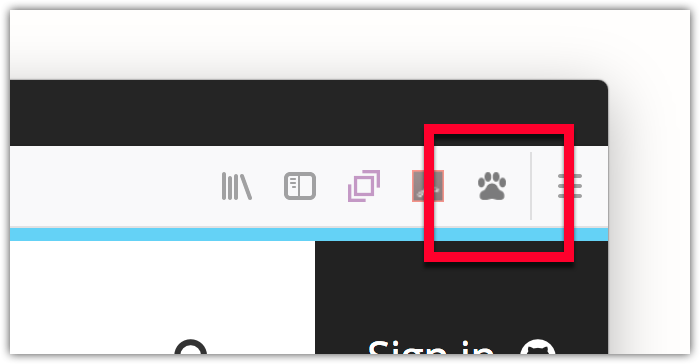
\includegraphics[width=0.5\linewidth]{img/browser-action.png}
  \caption{A button added via the \texttt{browserAction} WebExtension API}
  \label{img:browser-action}
\end{figure}

It should be able for custom qutebrowser extensions to add their own user
interface elements. However, this functionality is unlikely to be needed
when moving core functionality into plugins (which is the main focus of this
SA). Therefore, this API is currently out of scope.

\subsubsection{browserSettings}
\begin{quote}
Enables an extension to modify certain global browser settings.
\end{quote}

Extensions for qutebrowser should be able to modify its settings, and also
define their own options.

\subsubsection{browsingData}
\begin{quote}
Enables extensions to clear the data that is accumulated while the user is
browsing.
\end{quote}

No such functionality is currently implemented in qutebrowser, so this API is
out of scope.

\subsubsection{clipboard}
\begin{quote}
The clipboard API enables an extension to copy items to the system clipboard.
\end{quote}

Since qutebrowser extensions will have access to the Qt GUI library, no
equivalent to this module is needed. Qt provides the
\verb|QClipboard|\footnote{\url{http://doc.qt.io/qt-5/qclipboard.html}} class, which can
be used for equivalent functionality.

\subsubsection{commands}
\begin{quote}
Listen for the user executing commands that you have registered using the commands manifest.json key.
\end{quote}

This API is used to register custom keyboard shortcuts in WebExtensions. A
similar concept also exists in qutebrowser, where commands can either be bound
to keys (using the configuration), or executed in the commandline via \verb|:command|.

This API is important, since many core parts register commands in qutebrowser
(like \verb|:adblock-update| for the ad blocker). Thus, Extensions should be
able to register Python functions as commands.

\subsubsection{contentScripts}
\begin{quote}
With the contentScripts API, an extension can register and unregister scripts at runtime.
\end{quote}

Injecting custom JavaScript code into websites will be an useful feature for
custom plugins at a later stage, but isn't needed to move code out of
qutebrowser's core, as it's expected for internal JavaScript code to stay in the
core part. Thus, this module is currently out of scope.

Running JavaScript one-off snippets (triggered manually, rather than
automatically on page load) is already implemented in the tab API, and should be
trivial to expose to plugins.

\subsubsection{contextualIdentities, i18n, identity, idle, notifications, pkcs11, topSites}
\begin{quote}
contextualidentities: Work with contextual identities: list, create, remove, and update contextual identities.
\end{quote}
\begin{quote}
i18n: Functions to internationalize your extension. You can use these APIs to get localized strings from locale files packaged with your extension, find out the browser's current language, and find out the value of its Accept-Language header.
\end{quote}
\begin{quote}
identity: Use the identity API to get an OAuth2 authorization code or access token, which an extension can then use to access user data from a service which supports OAuth2 access (such as a Google or a Facebook account).
\end{quote}
\begin{quote}
idle: Find out when the user's system is idle, locked, or active.
\end{quote}
\begin{quote}
notifications: Display notifications to the user, using the underlying operating system's notification mechanism.
\end{quote}
\begin{quote}
pkcs11: The pkcs11 API enables an extension to enumerate PKCS\#11 security modules, and to make them accessible to the browser as sources of keys and certificates.
\end{quote}
\begin{quote}
topSites: Use the topSites API to get an array containing pages that the user has visited often and frequently.
\end{quote}

No such functionality is currently implemented in qutebrowser, so those modules
are out of scope.

\subsubsection{cookies}
\begin{quote}
Enables extensions to get and set cookies, and be notified when they change.
\end{quote}

Cookie access isn't fully exposed by the QtWebEngine
library\footnote{\url{http://doc.qt.io/qt-5/qwebenginecookiestore.html}}, so
it's currently not possible to implement this module.

\subsubsection{devtools}
\begin{quote}
The devtools.inspectedWindow API lets a devtools extension interact with the window that the developer tools are attached to.
\end{quote}

\begin{quote}
The devtools.network API lets a devtools extension get information about network requests associated with the window that the devtools are attached to (the inspected window).
\end{quote}

\begin{quote}
The devtools.panels API lets a devtools extension define its user interface inside the devtools window.
\end{quote}

Access to developer tools isn't exposed by the QtWebEngine library, so it's
currently not possible to implement this module.

\subsubsection{dns}
\begin{quote}
Enables an extension to resolve domain names.
\end{quote}

Since qutebrowser extensions will have access to the Qt GUI library, no
equivalent to this module is needed. Qt provides the
\verb|QDnsLookup|\footnote{\url{http://doc.qt.io/qt-5/qdnslookup.html}} class, which can
be used for equivalent functionality.

\subsubsection{downloads}
\begin{quote}
Enables extensions to interact with the browser's download manager. You can use this API module to download files, cancel, pause, resume downloads, and show downloaded files in the file manager.
\end{quote}

This module is needed for various core parts (such as the ad blocker, to
download filter lists).

\subsubsection{events, extensions, extensionTypes, permissions, runtime, types}
\begin{quote}
events: Common types used by APIs that dispatch events.
\end{quote}
\begin{quote}
extensions: Utilities related to your extension. Get URLs to resources packages with your extension, get the Window object for your extension's pages, get the values for various settings. Note that the messaging APIs in this module are deprecated in favor of the equivalent APIs in the runtime module.
\end{quote}
\begin{quote}
extensionTypes: Some common types used in other WebExtension APIs.
\end{quote}
\begin{quote}
permissions: Extensions need permissions to access more powerful WebExtension APIs. They can ask for permissions at install time, by including the permissions they need in the permissions manifest.json key. The main advantages of asking for permissions at install time are:
\end{quote}
\begin{quote}
runtime: This module provides information about your extension and the environment it's running in.
\end{quote}
\begin{quote}
types: Defines the BrowserSetting type, which is used to represent a browser setting.
\end{quote}

Those APIs are specific to the WebExtensions API, and thus irrelevant for
qutebrowser.

\subsubsection{find}
\begin{quote}
Finds text in a web page, and highlights matches.
\end{quote}

This functionality is already available as part of the \emph{tab API}, and
should be trivial to expose to plugins.

\fixme{define ``tab api''}

\subsubsection{history}
\begin{quote}
Use the history API to interact with the browser history.
\end{quote}

Accessing and manipulating the history might be an useful feature for future
user-contributed plugins, but is likely not needed for moving code out of
qutebrowser's core. Thus, the history module is currently out of scope.

\subsubsection{management}
\begin{quote}
Get information about installed add-ons.
\end{quote}

Extensions are currently not expected to interact with each other (even less so
when moving code out of the core), so this module is not needed.

\subsubsection{omnibox}
\begin{quote}
Enables extensions to implement customised behavior when the user types into the
browser's address bar.
\end{quote}

When adding custom commands, extensions also should be able to specify a
completion function, so users can use qutebrowser's autocompletion when typing
the extension's commands.

\subsubsection{privacy}
\begin{quote}
Access and modify various privacy-related browser settings.
\end{quote}

In qutebrowser, those settings (like
\verb|privacy.network.webRTCIPHandlingPolicy|) are exposed as normal qutebrowser
setttings (like \verb|content.webrtc_ip_handling_policy|), so there's no need
for a similar module in the plugin API.

\subsubsection{proxy}
\begin{quote}
Use the proxy API to proxy web requests. There are two different ways you can do this:
\end{quote}

No low-level networking access is possible via the QtWebEngine API, so this
module will not be implemented.

\subsubsection{search}
\begin{quote}
Retrieves search engines and executes a search with a specific search engine.
\end{quote}

Search engines are part of the main configuration in qutebrowser, so an
extension can trivially retrieve a search engine from there and execute a query
without the need for a dedicated API.

\subsubsection{sessions}
\begin{quote}
Use the sessions API to list, and restore, tabs and windows that have been closed while the browser has been running.
\end{quote}

While qutebrowser does have a session feature, access to it is not vital for a
plugin API, so this is currently out of scope.

\subsubsection{storage}
\begin{quote}
Enables extensions to store and retrieve data, and listen for changes to stored items.
\end{quote}

Having a simple way to persist data for extensions will be an useful feature for
third-party extensions, but is currently not needed when moving code out of the core.

\subsubsection{tabs, windows}
\begin{quote}
tabs: Interact with the browser's tab system.
\end{quote}
\begin{quote}
windows: Interact with browser windows. You can use this API to get information about open windows and to open, modify, and close windows. You can also listen for window open, close, and activate events.
\end{quote}

Various functionality already exists in qutebrowser as part of the ``tab API'',
which should be trivial to expose to the plugin API. Furthermore, the
\verb|tabs| and \verb|windows| modules contains various functionality to
retrieve tabs, which should be added to qutebrowser's plugin API.

\subsubsection{theme}
\begin{quote}
Enables browser extensions to update the browser theme.
\end{quote}

No dedicated theme feature exists in qutebrowser - instead, qutebrowser's user
interface can be customized using its configuration.

\subsubsection{webNavigation}
\begin{quote}
Add event listeners for the various stages of a navigation. A navigation consists of a frame in the browser transitioning from one URL to another, usually (but not always) in response to a user action like clicking a link or entering a URL in the location bar.
\end{quote}

This exposes various events such as \verb|webNavigation.onCompleted|. Those will
be exposed as part of the tab API in qutebrowser, as Qt signals such as \verb|load_finished|.

\subsubsection{webRequest}
\begin{quote}
Add event listeners for the various stages of making an HTTP request. The event listener receives detailed information about the request, and can modify or cancel the request.
\end{quote}

The \verb|webRequest| module allows extensions to intercept and change HTTP
network requests. Many of the fine-grained modifications exposed by
WebExtensions (such as \verb|onResponseStarted| to modify the network response)
are not available in the QtWebEngine API, so exposing them in qutebrowser's API
won't be possible. However, it's possible to intercept and block network
requests, and such functionality is critical to move components like the ad
blocker out from the core.

% Bestehende Lösungsansätze und Normen
%\section{Existing APIs}

% Kurzbeschreibung und Charakterisierung
% \section{Summary and Characerization}

% Defizite (Hinweise auf Weiterentwicklungs-, bzw. Verbesserungspotential)
%\section{Problems with existing solutions}  

% Bewertung (Evaluation)
\chapter{Evaluation}

% Kriterien (Wie wird bewertet?)
\section{Criteria}

\label{criteria}

There are various forces which affect design decisions for qutebrowser's plugin
API:

\begin{description}
\item[Qt APIs] qutebrowser is built on top of the QtWebEngine/QtWebKit
rendering engines (which of the two to use is user-configurable). To some
degree, the APIs exposed by those libraries also dictates how the API
qutebrowser can expose to plugins can look. The API to get the selected text
from a web page is an ideal example: The most straightforward API would be a
\py{def selection() -> str} method. However, JavaScript execution is needed to get
the selection, which is only available from Qt as a callback-based interface.
Thus, the plugin API will need to look like
\py{def selection(cb: Callable[[str], None]) -> None} --
in other words, the \py{selection} method will take a
callback function, which then gets called with the selected text.

\item[Internal qutebrowser code] One of the main goals (as per the task
description) of this SA is moving code from qutebrowser's core into internal
``plugins'' shipped alongside qutebrowser. Components which use general-purpose
APIs (like the adblocker, which needs to intercept network requests) can
conveniently moved out of the core, and result in plugin APIs which are also
usable for other purposes.

\item[Ideas for future plugins] While external plugins (contributed by the
qutebrowser community) are not the primary focus of this SA, a lot of use-cases
for plugins have been collected based on users' feature requests. Care should be
taken so the plugin API can also satisfy those use cases in the future.

\item[Other plugin APIs] There is a general consensus from browser vendors
around the WebExtension plugin API. Unfortunately, that API is unsuitable for
qutebrowser, for reasons explained in chapter \ref{unsuitable}. It can still
serve as a source for inspiration.

\item[Python and Qt] While some higher-level architectural decisions are
independent from the programming language used to implement them, what is
commonly considered a ``good'' API certainly depends on the underlying
programming language and the idioms used therein. Since qutebrowser's plugin API
is used from Python, it should aim to be ``Pythonic'' (i.e., adhering to Python
idioms\footnote{\url{https://blog.startifact.com/posts/older/what-is-pythonic.html}})
and also use features made available by Qt. As an example, a Pythonic API might
favor Python
decorators\footnote{\url{https://docs.python.org/3/glossary.html\#term-decorator}}
over inheritance to set up plugin hooks; or a Qt API might prefer Qt's
signals/slots
facility\footnote{\url{https://doc.qt.io/qt-5/signalsandslots.html}} over a
callback-based API.
\end{description}


% Schlussfolgerungen, eigener Lösungsansatz
\section{Conclusion}


% Umsetzungskonzept (des eigenen Lösungsansatzes)
\chapter{Concept}

% Grobe Beschreibung des eigenen Lösungskonzepts
\section{Summary}

% z.T. Wiederholung im Groben, z.T. Verweise auf Teil II-Kapitel
\section{...}


% Resultate, Bewerung und Ausblick
\chapter{Results}

% Zielerreichung
\section{Achievement of Objectives}

% Ausblick: Weiterentwicklung (nur wichtigste Punkte)
\section{Future Work}

% Persönliche Berichte
\section{Personal Review}

% Dank
\section{Thanks}



% Teil II SW-Projektdokumentation ("klassisches" RUP 2/HSR)  
\part{Project Documentation}


% Vision (ev. auf Kapitel 1.1 verweisen)
\chapter{Vision}


% Anforderungsspezifikation
\chapter{Requirements Specification}

% Anforderung an die Arbeit
\section{Requirements of the Project}

% Use Cases (Success Scenario / Success Diagram)
\section{Use Cases}

% System-Sequenzdiagramme
\section{System Sequence Diagrams}

% Weitere Funktionen, die nicht erfasst wurden
\section{Further Functionality}

% Nicht-funktionale Anforderungen (Rahmbenbedingungen, evtl. Verweis auf 1.3)
\section{Non-functional Requirements}

% Detailspezifikation
\section{Detailed Specification}


% Analyse (Business Model)
\chapter{Analysis}

% Domain Modell, Klassendiagramme (konzeptionell)
\section{Domain Model}

% Objektkatalog (Beschreibung der Konzepte, bzw. Entitätsmengen)
\section{Objects}


% Design (Entwurf)
\chapter{Design}

% Architektur
\section{Architecture}

% Objektkatalog (Klassenkonzepte, Verantwortlichkeiten und Konsistenzbedingungen)
\section{Objects}

% Package- und Klassendiagramme (konzeptionell)
\section{Packages and Classes}

% Sequenzdiagramm, UI Design
\section{Sequence Diagrams}


% Implementation (Entwicklung)
\chapter{Implementation and Test}

% Implementation: Erläuterungen wichtiger konkreter Klassen
\section{Important Classes}

% Automatische Testverfahren
\section{Automated Testing}

% Manuelle Testverfahren, etc.
\section{Manual Testing}


% Resultate und Weiterentwicklung
\chapter{Results and Future Work}

% Resultate (ev. nach oben in Teil I Kap. 5 eingleidern)
\section{Results}

% Möglichkeiten der Weiterentwicklung
\section{Possible Future Work}

% Vorgehen (welche Mögl. würde man nun wie weiterentwickeln?)
\section{Future Approach}


% Projektmanagement (Planung, Soll)
\chapter{Project Management}

% Prototypen, Releases, Meilensteine
\section{Prototypes, Releases, Milestone}

% Team, Rollen und Verantwortlichkeiten
\section{Team and Roles}
\emph{Florian Bruhin} is both the primary maintainer of qutebrowser and the
author of this student research project. He has been working on qutebrowser since
December 2013 and started studying Computer Science at HSR in 2016.

Professor \emph{Stefan Keller}, institute partner at the Institute for Software
(IFS) at HSR is the advisor for this project.

The qutebrowser community is not directly involved in this research project, but
is the primary audience of the resulting work. It has also contributed many
ideas and use cases for future
plugins\footnote{\url{https://github.com/qutebrowser/qutebrowser/issues/30}}.

\label{fiete}
\emph{Fritz Reichwald} (fiete201\footnote{\url{https://github.com/fiete201}})
is a long-time qutebrowser user who is working on migrating qutebrowser's
documentation system from asciidoc\footnote{\url{http://asciidoc.org/}} (which
is deprecated) to the Sphinx\footnote{\url{http://www.sphinx-doc.org/}}
documentation generator. This change was
planned\footnote{\url{https://github.com/qutebrowser/qutebrowser/issues/345}}
since December 2014, so his help with tackling this is very much appreciated.
This project will benefit from his work, as Sphinx, unlike asciidoc, is a
very good fit for documenting APIs. His work is clearly marked as such in this
documentation.

% Aufwandschätzung, Zeitplan, Projektplan
\section{Project Schedule}
% Risiken
\section{Risks}
% Prozessmodel
\section{Process Model}


% Projektmonitoring (Ist-Beschreibung, so ist es passiert)
\chapter{Project Monitoring}
% Soll-Ist-Zeit-Vergleich
\section{Allocated/Actual Time}
% Codestatistik (Zeilen: Kommentare, Klassen, Packages)
\section{Code Statistics}


\chapter{Software Documentation}
% Maybe separate (Sphinx)



\part{Appendices}


\chapter{Glossary and Abbreviations}

Test \citep{yapproach}

\renewcommand{\bibname}{\chapter{Literature and Sources}}
\bibliographystyle{IEEEtranN}
\bibliography{bibliography}

\end{document}
